\section{Работа поддетекторов}
\subsection{SVD}


\begin{wrapfigure}{r}{0.5\textwidth}
    \centering
    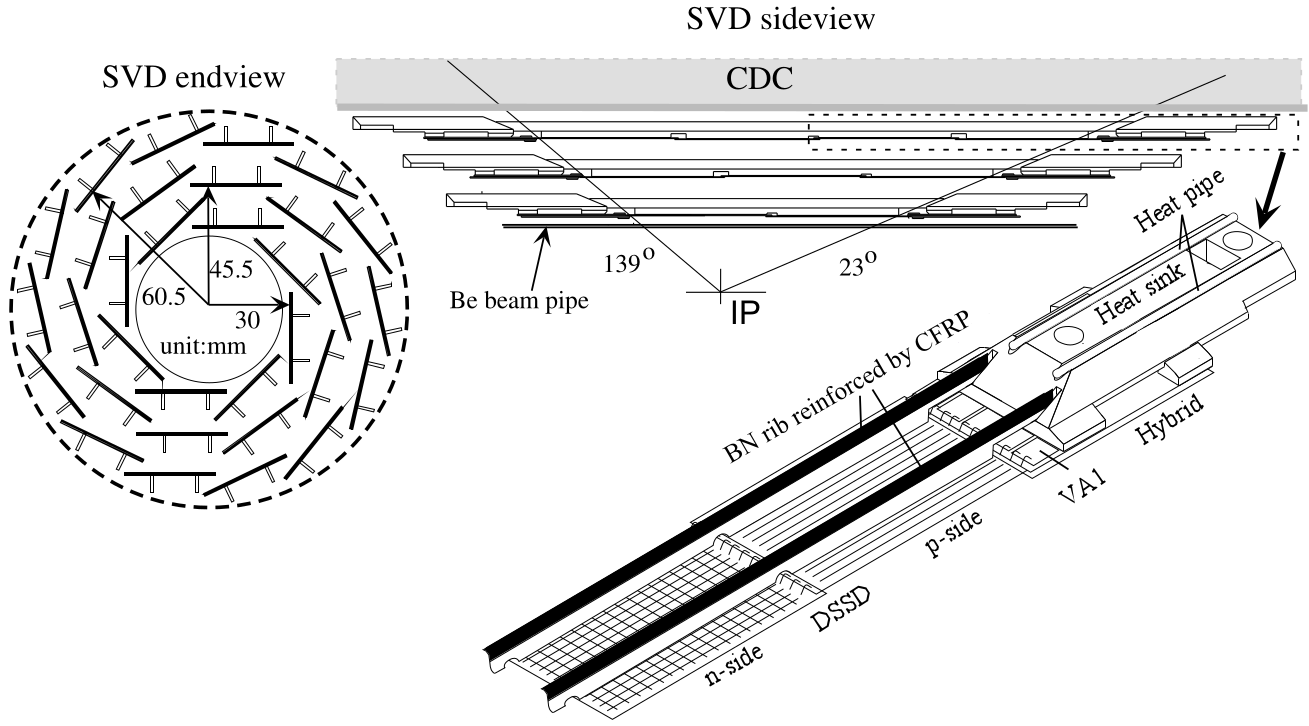
\includegraphics[width=0.48\textwidth]{img/SVD.png}
    \caption{SVD}
    \label{the:SVD}
\end{wrapfigure}

Кремниевый вершинный детектор, расположенный ближе всего к точке взаимодействия, 
предназначен для определения её точного местоположения. 
Он состоит из тонких слоёв, покрывающих угол от $23^\circ$ до $139^\circ$, 
расположенных внахлёст и разбитых на секции, в которых при пролёте частицы 
образуется электронно-дырочная пара. Благодаря большому сечению взаимодействия, 
высокой плотности материала и низкой энергии взаимодействия, твердотельные 
счётчики способны работать точно для широкого диапазона энергий частиц.
Всё это позволяет определять точку взаимодействия с точностью до 100 мкм. 
Однако, несмотря на более высокую точность по сравнению с газовыми детекторами, 
установка большого числа слоёв затруднена из-за возможного сильного отклонения 
трека в результате многократного взаимодействия с плотными кристаллами кремния.



